\documentclass[bare_jrnl_transmag]{subfiles}
\begin{document}

\subsection{Vision Relative Odometry Implementation}

<<<<<<< HEAD
Visual odometry involves extracting information from a series of images in order to estimate the pose and position of a camera. The dataset provides 30 frames per second stereo images allowing for 3D localization. OpenCV was used for the image extraction and processing \cite{opencv}. The overall process is outlined in \ref{fig:vio_process}.

\begin{figure}[H]
    \centering
    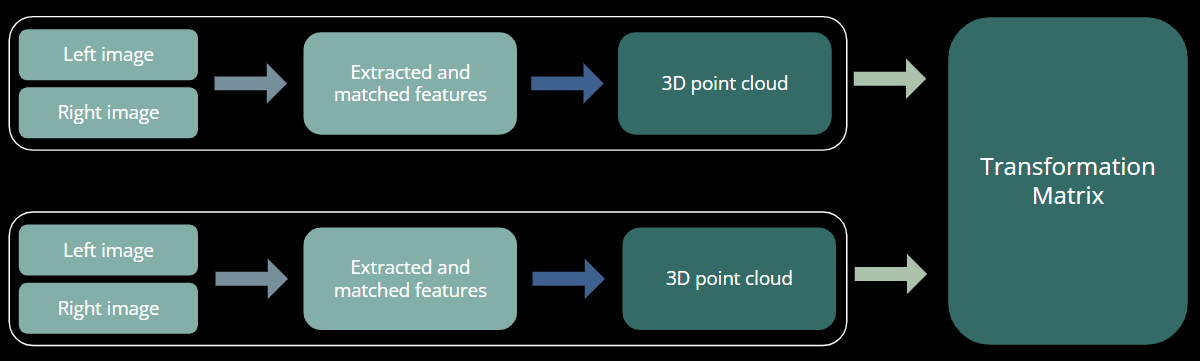
\includegraphics[width=1\linewidth]{figures/VIO_process.png}
    \caption{High-level process for relative visual odometry.}
    \label{fig:vio_process}
\end{figure}

Image features were first extracted from left and right pairs of images at a given time step. The Scale-Invariant Feature Transform (SIFT) feature extraction algorithm was used. The features of the two images were then matched to ensure the same points in both are compared. The Fast Library for Approximate Nearest Neighbors (FLANN) matcher was used to create feature matches between the two images.  Random sample consensus (RANSAC) was then used to filter these matches, only preserving the highest quality matches. These steps were repeated for the previous time step, and the filtering was again applied, this time between the left images of the previous and current time step. This ensured that the two point clouds generated contain the same points such that the transformation between them can be found. \newline

With the same features identified in both the left and right images, a 3D point cloud was generated by using triangulation to find the location of the points in 3D space. The image was first undistorted to match a pinhole camera model. This was done by using the intrinsic transformation matrix provided in the calibration data. The point clouds at sequential time steps were then generated using triangulation, producing two point clouds with ideally the same points. This process is visualized in Appendix \ref{app:vision_diagrams}. \newline

To find the transformation between these two point clouds, outlier points, such as points behind the camera, were removed. A custom iterative method was then used to find the transformation. A first guess transformation was applied to the previous time step's point cloud known as the source. The distances between the points in the source were now compared to the current time step's (destination) point cloud. Weights for each point were generated that are inversely proportional to the distances. The centroid of the point cloud was then found using the weights, and the centroids were aligned. The weighted covariance was found and PCA was used to obtain the principal components of the covariance. These principal axes were then aligned, and the rotation required to do this is saved was the rotation matrix. This rotation could then be applied to the source point cloud, and the translation between them was found through simple subtraction. This transformation was then fed back to the start of the process, and was repeated until the transformation matrix converged. A graphic visualizing alignment is shown in Appendix \ref{app:vision_diagrams}. \newline

The system returns a relative transformation vector, t, and rotation matrix R. The relative rotation was not passed to the Kalman filter as another inertial-only orientation filter (Madgwick) was used. The drone's previous pose estimate from the Kalman filter was used to convert the relative translation into the world frame before using it in the update step.

\end{document}